\documentclass{standalone}
\usepackage[utf8]{inputenc}
\usepackage[compat=0.6]{yquant}
\usepackage{newtxmath}
\usetikzlibrary{quotes}
\usetikzlibrary{calc}
\usepackage{xcolor}
\useyquantlanguage{groups}


\begin{document}

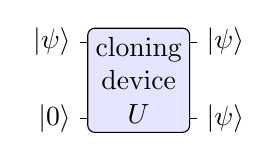
\begin{tikzpicture}
    \begin{yquant*}
    qubit {$|\psi\rangle$} in;
    qubit {$|0\rangle$} q;

    [shape=yquant-rectangle, rounded corners=.25em, fill=blue!10, y radius=10pt]
    box {cloning\\device\\$U$} (in, q);

    output {$|\psi\rangle$} in;
    output {$|\psi\rangle$} q;
    \end{yquant*}
    \end{tikzpicture}

\end{document}